% lintrans - The linear transformation visualizer
% Copyright (C) 2021-2022 D. Dyson (DoctorDalek1963)

% This program is licensed under GNU GPLv3, available here:
% <https://www.gnu.org/licenses/gpl-3.0.html>

\documentclass[../development.tex]{subfiles}

\begin{document}

\subsubsection{Fixing an animation crash\label{development:fixing-bugs-and-adding-polish:fixing-an-animation-crash}}

The scaling logic in \ref{development:visualizing-matrices:preserving-determinants} creates a matrix $\mathbf{A}$ which is the start matrix plus some proportion of the difference between the target and start matrices. It then defines matrix $\mathbf{B}$ to be the matrix A normalised to have a determinant of 1. We then divide by $\det(\mathbf{B})$ to get matrix $\mathbf{C}$, which we then render.

This works very well for most matrices, but if we're animating from $\mathbf{I}$ to $-\mathbf{I}$ for example, then we can get the following problem:

When we're halfway through the animation, $p = \frac{1}{2}$.
\begin{align*}
\mathbf{A} &= \mathbf{S} + p (\mathbf{T} - \mathbf{S})\\
&= \mathbf{I} + \frac{1}{2} (-\mathbf{I} - \mathbf{I})\\
&= \mathbf{I} + \frac{-1}{\cancel{2}} \cancel{2} \mathbf{I}\\
&= \mathbf{I} - \mathbf{I} = \mathbf{0}
\end{align*}

I'm using $\mathbf{I}$ as an example here, but this can happen with the right $p$ for many matrix pairs. Since $\mathbf{A} = \mathbf{0}$, $\det(\mathbf{A}) = 0$. We check for this case already when we find $c$:

%: f7a91cdc35695f8fb9269b17bc103e42578072bd
%: src/lintrans/gui/main_window.py:367-370 noscopes

But if $\det(\mathbf{A}) = 0$, then $c = 0$ and $\det(\mathbf{B}) = 0$, so we also need to check that before we divide by it.

Old:

%: f7a91cdc35695f8fb9269b17bc103e42578072bd
%: src/lintrans/gui/main_window.py:383-384 noscopes

New:

%: 4383808a4cc29d192c55aca56161d8affda8c9a7
%: src/lintrans/gui/main_window.py:384-391 noscopes

This change fixes a division by zero bug, which eliminates a possible crash here.

\subsubsection{Limiting parallel lines\label{development:fixing-bugs-and-adding-polish:limiting-parallel-lines}}

If you try to render a matrix like \texttt{0.01Irot(45)}, then the app ends up drawing as many parallel lines as it can physically fit in the viewport. This leads to a lot of lag, especially when zoomed out far. To fix this, I just introduced a maximum number of parallel lines. I chose 150 as a number that was big enough to have enough parallel lines for matrices that need a lot, while also causing virtually no lag.

%: bd9aaa2e3037214f65d0fc1d12d67db35af0e5ec
%: src/lintrans/gui/plots/classes.py:169

%: bd9aaa2e3037214f65d0fc1d12d67db35af0e5ec
%: src/lintrans/gui/plots/classes.py:230-277

The idea behind this code is just to limit the maximum number of parallel lines that get drawn. It works perfectly for oblique lines, but there's a small bug for orthogonal lines that I never noticed. I just forgot to test it.

On lines 234 and 252, I call the built-in \pyinline{max()} function with the maximum number of parallel lines and the total number of lines that could fit in the viewport. This should be a call to \pyinline{min()} instead. I fixed this before releasing it for my end users, but it took an embarrassingly long time to notice something this simple.

\begin{figure}[H]
	\hspace{0.005\linewidth}
	\centering
	\begin{minipage}{0.48\linewidth}
		\centering
		\begin{figure}[H]
			\centering
			\includegraphics[width=\linewidth]{development/bd9aaa2e3037214f65d0fc1d12d67db35af0e5ec/old.png}
			\caption{The old version with too many parallel lines.}
			\label{fig:development:bd9aaa2e3037214f65d0fc1d12d67db35af0e5ec:old.png}
		\end{figure}
	\end{minipage}%
	\hspace{0.015\linewidth}
	\begin{minipage}{0.48\linewidth}
		\centering
		\begin{figure}[H]
			\centering
			\includegraphics[width=\linewidth]{development/bd9aaa2e3037214f65d0fc1d12d67db35af0e5ec/new.png}
			\caption{The fixed version with a maximum number of parallel lines.}
			\label{fig:development:bd9aaa2e3037214f65d0fc1d12d67db35af0e5ec:new.png}
		\end{figure}
	\end{minipage}
	\hspace{0.005\linewidth}
	\vspace{-1em}
\end{figure}

\subsubsection{Giving focus to the expression box\label{development:fixing-bugs-and-adding-polish:giving-focus-to-the-expression-box}}

It would be quite nice to be able to just start typing an expression after defining a matrix or changing display settings. To do this, we can simply set the app's focus on the expression box after either of these actions.

Additionally, it would be nice to update the render buttons at the same time. That would allow the user to use a matrix in an expression, then define it, and be able to render the expression as soon as they close the dialog (assuming the expression is valid).

%: bd7f8ba18266a8a095549d815dcfe6f24de514b6
%: src/lintrans/gui/main_window.py:438-446,454-459

\subsubsection{Fixing a crash when animating singular matrices in sequence\label{development:fixing-bugs-and-adding-polish:fixing-a-crash-when-animating-singular-matrices-in-sequence}}

If we have a matrix $\mathbf{A}$ defined as $\begin{pmatrix}1 & 2\\ 1 & 2\end{pmatrix}$, then when we try to render \texttt{A\^{}-1}, we get a pop-up dialog box saying that we can't take the inverse of a singular matrix. This is good, since if NumPy just took the inverse blindly, it would crash. When we try to animate \texttt{A\^{}-1}, we get the same pop-up box. When we try to use it in an animation sequence, however, like \texttt{rot(45),A\^{}-1}, we don't check if each element of the sequence for singularity, so NumPy takes the inverse blindly and the whole app crashes. This is bad.

To fix this, we can simply catch the error when trying to evaluate the element in the sequence.

%: 8db0df1d9d6a1be1f15a6f705e779d982db9ee29
%: src/lintrans/gui/main_window.py:300-310

\subsubsection{Allowing animations to be cancelled\label{development:fixing-bugs-and-adding-polish:allowing-animations-to-be-cancelled}}

Currently, if you try to reset the viewport partway through an animation, it just resets the basis vectors for a tick, but then they start moving again, because the animation loop is still running. To fix this, we can track whether we should be animating using an instance variable, set it to false when the user hits reset, and break out of the animation loop when it's false.

% Ideally, my snippet processing code would handle the scopes of these snippets automatically, but
% some of them need to share scopes, which would be more effort to implement than it's probably worth

%: b665bc59ec99664ed7b2c17f94e76ae49c6eb331
%: src/lintrans/gui/main_window.py:45-46,269-274,292,304-329,360,365-370,429

Here, \pyinline{self.animating_sequence} is whether a sequence is being animated, and \pyinline{self.animating} is whether an individual matrix is currently being animated. An individual matrix means a matrix on its own, or a single element in a sequence. That means that \pyinline{self.animating} can be set and unset multiple times in a single sequence.

\subsubsection{Validating expression input\label{development:fixing-bugs-and-adding-polish:validating-expression-input}}

The user can only render or animate an expression if it's actually valid, as discussed in \S\ref{development:matrices-backend:simple-matrix-expression-validation}, and the render and animate buttons will be greyed out if the expression is invalid. But they can still type anything into the box.

It was at this point that I learned about the \pyinline{QValidator} class\cite{qt5-docs-qvalidator}. This class allows me to control what the user can actually type. Using the implementation below, they can only enter characters that are allowed in valid matrix expressions.

%: f73575c017548d754e4171449344a52cb44b7ef4
%: src/lintrans/gui/main_window.py:125

%: f73575c017548d754e4171449344a52cb44b7ef4
%: src/lintrans/gui/validate.py

I also then added validators to the definition dialogs, to make sure that users can only enter valid input. Qt5 provides some basic validators already, for things like integers and floating point numbers (called \mintinline{C++}{double} in C++, equivalent to \pyinline{float} in Python).

%: a2fd14b99fa752a18b42352a01142ffbc2600570
%: src/lintrans/gui/dialogs/define_new_matrix.py:213,225-240,299,314-317,358,372-375 noscopes

\subsubsection{Adding keyboard shortcuts\label{development:fixing-bugs-and-adding-polish:adding-keyboard-shortcuts}}

Keyboard shortcuts are often very useful and can make the process of using software much more efficient if you get good at using the shortcuts. On this note, I decided to add keyboard shortcuts to the display settings dialog.

Qt5 lets you use a \texttt{\&} character in the text of a widget to act on the letter following it. This letter becomes underlined in the text, and the user can hold \texttt{Alt} and press this letter to activate the widget. I also want to be able to toggle the checkboxes by just pressing the letter without holding \texttt{Alt}, so I had to implement this myself with a dictionary and custom override of \pyinline{keyPressEvent()}.

%: 67d43a364ee2605b95b8caca9f1e4eb714cbb7c6
%: src/lintrans/gui/dialogs/settings.py:63-155,188-210

\subsubsection{Centering text in the determinant parallelogram\label{development:fixing-bugs-and-adding-polish:centering-text-in-the-determinant-parallelogram}}

The text in the determinant parallelogram is the numerical value of the determinant. Currently, it's not centered. It's drawn by just writing the text at a point, chosen to be the centre of the parallelogram. The \pyinline{QPainter} class uses this point as the start of the baseline of the text, so it's effectively the bottom left corner.

%: 67d43a364ee2605b95b8caca9f1e4eb714cbb7c6
%: src/lintrans/gui/plots/classes.py:419-428

Obviously, this text will look better if it's centered. To do this, we can create a bounding rectangle around the parallelogram and get the painter to draw the text in the centre of that rectangle.

We build the rectangle by getting the coordinates of each vertex of the parallelogram. Then the top left corner is the minimum $x$ coordinate with the maximum $y$ coordinate, and the bottom right corner is the maximum $x$ with the minimum $y$.

%: 9550416c0b273b16c90eb8d6319f5e17493ef9a8
%: src/lintrans/gui/plots/classes.py:419-447

\begin{figure}[H]
	\hspace{0.05\linewidth}
	\centering
	\begin{minipage}{0.35\linewidth}
		\centering
		\begin{figure}[H]
			\centering
			\includegraphics[width=\linewidth]{development/9550416c0b273b16c90eb8d6319f5e17493ef9a8/old.png}
			\caption{Text not centered.}
			\label{fig:development:9550416c0b273b16c90eb8d6319f5e17493ef9a8:old.png}
		\end{figure}
	\end{minipage}%
	\hspace{0.2\linewidth}
	\begin{minipage}{0.35\linewidth}
		\centering
		\begin{figure}[H]
			\centering
			\includegraphics[width=\linewidth]{development/9550416c0b273b16c90eb8d6319f5e17493ef9a8/new.png}
			\caption{Text centered.}
			\label{fig:development:9550416c0b273b16c90eb8d6319f5e17493ef9a8:new.png}
		\end{figure}
	\end{minipage}
	\hspace{0.05\linewidth}
	\vspace{-1em}
\end{figure}

\subsubsection{Defining matrices as expressions\label{development:fixing-bugs-and-adding-polish:defining-matrices-as-expressions}}

Currently, you can \enquote*{define} a matrix in terms of an expression, but it doesn't really define the matrix like that. Instead, it evaluates the expression immediately, and assigns that numerical result to the name you specified. It would be much better if the matrix could be actually defined as the expression, and then evaluated only when it needs to be used. Then, the user could have a matrix $\mathbf{M}$ defined as something like \texttt{0.5A\^{}-1rot(45)B}, and it would always have that value, even if the user has changed the definition of $\mathbf{A}$ or $\mathbf{B}$ since defining $\mathbf{M}$.

To do this, I'll have to completely change how matrices are stored and retrieved. The \pyinline{MatrixWrapper} class contains a dictionary \pyinline{self._matrices}, which currently maps \pyinline{str} to \pyinline{Optional[MatrixType]}, meaning that a matrix could be a $2 \times 2$ NumPy array, or nothing. I'm going to change this type to \pyinline{Optional[Union[MatrixType, str]]}. This means that if a matrix exists, then it's either a $2 \times 2$ NumPy array or a string. We then check which one it is when we retrieve the matrix, and act accordingly. If it's an expression, then we evaluate and return the numerical result.

Here's the relevant parts of the old \pyinline{MatrixWrapper} class:

%: 9550416c0b273b16c90eb8d6319f5e17493ef9a8
%: src/lintrans/matrices/wrapper.py:35-46,91-161

And here's the new version, which supports matrices defined as expressions:

%: 01e866a74cf0f02ecba6438763d43e6eb90fe218
%: src/lintrans/matrices/wrapper.py:38-49,94-193

One of the more subtle things added here is on lines 189-191. When checking if an expression is valid in the context of the wrapper, we have to make sure all the referenced matrices are actually defined, but if any of those matrices are defined as an expression, then obviously that expression has to be valid as well. This recursion means that all references to matrices must be valid, even traversing down through matrices that are defined as expressions.

I also added some unit tests to automatically test this new feature.

%: 239bcbfd1dde3f7623318d03e8544dd67dc02e3d
%: tests/matrices/matrix_wrapper/test_setitem_and_getitem.py:42-199

%: ea00703f19c13af86c39ae30170569819937fa31
%: tests/matrices/matrix_wrapper/test_misc.py

\pytestScreenshot{ea00703f19c13af86c39ae30170569819937fa31}

I then had to fix a small bug where the \pyinline{DefineAsAnExpressionDialog} would evaluate the expression before assigning it, so I had to change that to just assign the test instead.

%: 54e10dbfd3a1f3a962955c7fa3908848f5bd95b0
%: src/lintrans/gui/dialogs/define_new_matrix.py:388-391

I also created a virtual method in the \pyinline{DefineDialog} superclass, which standardised how dialogs load a matrix when it's selected in the drop-down. The numerical and visual definition dialogs already did this, but it was inconsistent, so I made it the same across all subclasses, and added it to the expression dialog.

%: d1b60b20666ab9297cdbf675b6226587fd2e417f
%: src/lintrans/gui/dialogs/define_new_matrix.py:98-103,134-143,352,386-393

Unfortunately, my initial implementation of this had a few bugs, and I noticed a few hours later that if you first define $\mathbf{A}$ as anything concrete, then you can define $\mathbf{A}$ to be the expression \texttt{A}. Then, when you put it in the expression box, the app just crashes. This is because it recurs forever, since it doesn't realise that the definition of $\mathbf{A}$ is self-referential\footnote{Obviously it doesn't actually recur forever, but Python stops recursion after 1000 levels and crashes the program.}.

To fix this, I can check that the expression is valid and that it doesn't contain itself before assigning the expression to the matrix name.
% TODO: Reference future sss in footnote about circular references

%: 742e0955e344deab2c9302ba9a6c7298ec4583d4
%: src/lintrans/gui/dialogs/define_new_matrix.py:395-398

I also added this logic directly to the wrapper, so that there was no risk of me creating this kind of bug elsewhere.

%: e56a5a90034f8335b046dd1bf76321eb48892050
%: src/lintrans/matrices/wrapper.py:145-151

While I was working with expressions so much, I realised that defining a matrix as a rotation was a bit redundant when you can just use an expression like \texttt{rot(45)}. I spoke to the teacher that's going to use \texttt{lintrans} when it's finished, and she said that radians aren't really needed. The radians checkbox was the only unique part of the \pyinline{DefineAsARotationDialog} class. Since it's not important, I decided to remove the whole dialog.

\end{document}
